\documentclass[11pt, letterpaper, titlepage]{article}

\usepackage[utf8]{inputenc}
\usepackage[margin=1in]{geometry}
\usepackage{listings}
\usepackage{hyperref}
\usepackage{graphicx}
\usepackage{color}

\lstset{language=Python}
\pagenumbering{roman}

\begin{document}
\author{Hayden Jones}
\title{QuIN Lab Automation Guide \\ {\normalsize Version 2.0.2}}
\maketitle
%%%%%%%%%%%%%%%%%%%%%%%%%%%%%%%%%%%%%%%%%%%%%%%%%%%%%%%%%%%%%%%%%%%%%%%%%%%%%%%
\section*{Preface} \label{preface}
\addcontentsline{toc}{section}{Preface}
This guide is intended to provide instructions and assistance in the following categories:
\begin{itemize}
    \item Software Installation
    \item Hardware Operation
    \item Software Operation
    \item Troubleshooting
    \item Programming
\end{itemize}
%%%%%%%%%%%%%%%%%%%%%%%%%%%%%%%%%%%%%%%%%%%%%%%%%%%%%%%%%%%%%%%%%%%%%%%%%%%%%%%
\newpage
\section*{Changes} \label{changes}
\addcontentsline{toc}{section}{Changes}
The Version 2.0.2 Updates are as follows:
\begin{itemize}
%    \item General
%    \begin{itemize}
%        \item {\color{green} ADDED:} 
%        \item {\color{yellow} CHANGED:}
%        \item {\color{red} REMOVED:}
%    \end{itemize}
%    \item Software Installation
%    \begin{itemize}
%        \item {\color{green} ADDED:}
%        \item {\color{yellow} CHANGED:}
%        \item {\color{red} REMOVED:}
%    \end{itemize}
%    \item Hardware Operation
%    \begin{itemize}
%        \item {\color{green} ADDED:}
%        \item {\color{yellow} CHANGED:}
%        \item {\color{red} REMOVED:}
%    \end{itemize}
    \item Software Operation
    \begin{itemize}
%        \item {\color{green} ADDED:}
        \item {\color{yellow} CHANGED:} Updates to reflect software updates.
%        \item {\color{red} REMOVED:}
    \end{itemize}
%    \item Troubleshooting
%    \begin{itemize}
%        \item {\color{green} ADDED:}
%        \item {\color{yellow} CHANGED:}
%        \item {\color{red} REMOVED:}
%    \end{itemize}
%    \item Programming
%    \begin{itemize}
%        \item {\color{green} ADDED:}
%        \item {\color{yellow} CHANGED:}
%        \item {\color{red} REMOVED:}
%    \end{itemize}
\end{itemize}
%%%%%%%%%%%%%%%%%%%%%%%%%%%%%%%%%%%%%%%%%%%%%%%%%%%%%%%%%%%%%%%%%%%%%%%%%%%%%%%
\newpage
\tableofcontents
%%%%%%%%%%%%%%%%%%%%%%%%%%%%%%%%%%%%%%%%%%%%%%%%%%%%%%%%%%%%%%%%%%%%%%%%%%%%%%%
\newpage
\pagenumbering{arabic}
\section{Software Installation} \label{softwareinstallation} % 1
This section details the installation of necessary software for running the automation.
%%%%%%%%%%%%%%%%%%%%%%%%%%%%%%%%%%%%%%%%%%%%%%%%%%%%%%%%%%%%%%%%%%%%%%%%%%%%%%%
\subsection{Anaconda} \label{anaconda} % 1.1
For our project, we are using Anaconda 3 64-bit as our Python distribution.
%%%%%%%%%%%%%%%%%%%%%%%%%%%%%%%%%%%%%%%%%%%%%%%%%%%%%%%%%%%%%%%%%%%%%%%%%%%%%%%
\subsubsection{Downloads} % 1.1.1
The Anaconda distribution can be downloaded \href{https://www.continuum.io/downloads}{here}.
The Python version number is different from the Anaconda version number, but we only care about the Python version number.
The download required is ``Python 3.5 version 64-bit Installer''.
%%%%%%%%%%%%%%%%%%%%%%%%%%%%%%%%%%%%%%%%%%%%%%%%%%%%%%%%%%%%%%%%%%%%%%%%%%%%%%%
\subsubsection{Install Guide} % 1.1.2
\begin{enumerate}
    \item Run the executable downloaded as administrator.
    \item Select ``Next'', then ``I Agree''.
    \item Select``Install for: All Users'', then ``Next''.
          All other settings can be left default.
    \item Select ``Yes'' to administrator privileges.
    \item Select ``Next''.
    \item Ensure both checkboxes are checked. Then select ``Install''.
    \item Wait for the installation process to finish.
    \item Select ``Next''.
    \item Uncheck ``Learn more about Anaconda Cloud'' then ``Finish''.
    \item Right-click the start menu icon, then click ``System''.
    \item Click ``Advanced System Settings''.
    \item Click ``Environment Variables'' (under the ``Advanced'' tab).
    \item Click on ``PATH'' then ``Edit''.
    \item If there are no Anaconda directories specified, we need to add them.
    \begin{enumerate}
        \item Click ``New'' then type ``C:\textbackslash''. Make two entries.
        \item Click ``Browse...'' then navigate to and select the installation directory for Anaconda.
        \subitem They should look similar to Figure \ref{fig:anaconda_path}.
        \begin{figure}[h]
            \begin{center}
            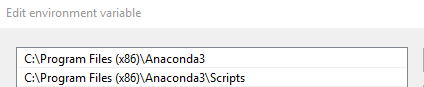
\includegraphics[scale=1.0]{anaconda_path.png}
            \caption{PATH Variables for Anaconda 3}
            \label{fig:anaconda_path}
            \end{center}
        \end{figure}
        \item Restart the computer.
    \end{enumerate}
\end{enumerate}
%%%%%%%%%%%%%%%%%%%%%%%%%%%%%%%%%%%%%%%%%%%%%%%%%%%%%%%%%%%%%%%%%%%%%%%%%%%%%%%
\subsubsection{Verify Installation} % 1.1.3
In order to check that Anaconda is installed correctly, and has proper PATH variables, open a command prompt and enter ``python''.
It should look very similar to Figure \ref{fig:anaconda_prompt}.
\begin{figure}[h]
    \begin{center}
    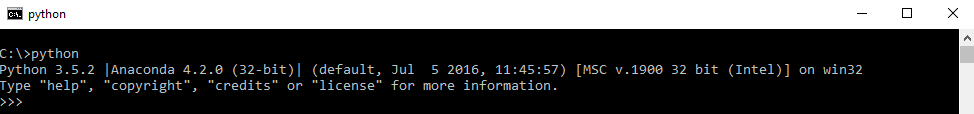
\includegraphics[scale=.65]{anaconda_prompt.png}
    \caption{Anaconda Python in Command Prompt}
    \label{fig:anaconda_prompt}
    \end{center}
\end{figure}
%%%%%%%%%%%%%%%%%%%%%%%%%%%%%%%%%%%%%%%%%%%%%%%%%%%%%%%%%%%%%%%%%%%%%%%%%%%%%%%
\subsection{Anaconda Packages} \label{anacondapkgs} % 1.2
These are the packages that must be installed after Anaconda is installed.
%%%%%%%%%%%%%%%%%%%%%%%%%%%%%%%%%%%%%%%%%%%%%%%%%%%%%%%%%%%%%%%%%%%%%%%%%%%%%%%
\subsubsection{Downloads} % 1.2.1
Open the QuIN Lab Google Drive, navigate to ``Hayden Jones\textbackslash Automation''.
Download ``wxpython-phoenix.zip'', and ``source-code.zip''.
It is safe to rename ``source-code.zip'' to something more descriptive; however ``wxpython-phoenix.zip'' cannot be renamed.
%%%%%%%%%%%%%%%%%%%%%%%%%%%%%%%%%%%%%%%%%%%%%%%%%%%%%%%%%%%%%%%%%%%%%%%%%%%%%%%
\subsubsection{Install Guide} % 1.2.2
\begin{enumerate}
    \item Extract the downloaded zips to a folder on the desktop.
    \item Open an elevated command prompt.
        \subitem An elevated command prompt is a command prompt in administrator mode.
    \item Navigate in the command prompt to the desktop.
        \subitem You can do this by entering ``cd\textbackslash'', then ``cd \textless{}dir\_name\textgreater''.
    \item Enter the following commands consecutively, entering ``y'' when prompted:
    \begin{lstlisting}[frame=single]
conda install pyserial
conda install git
conda install patch
conda update -n root conda-build
python -m pip install PyVISA
python -m pip install thorlabs_apt
python -m pip install -U --pre -f \
    https://wxpython.org/Phoenix/snapshot-builds/ wxPython_Phoenix
python -m pip install pyautoit
python -m pip install --upgrade \
    https://github.com/jacexh/pyautoit/archive/master.zip
    \end{lstlisting}
    \item Note that the URLs in the wxPython Phoenix and PyAutoIt installations commands should be part of the same command that starts with ``python -m pip install''.
    \item Close the command prompt.
    \item Open Windows Explorer and navigate to the Anaconda installation directory.
    \item Open ``pkgs\textbackslash thorlabs\_apt-0.1-py35\_0\textbackslash Lib\textbackslash site-packages\textbackslash thorlabs\_apt''.
    \item Edit core.py with a Python IDE, Notepad++, or other similar program.
        \subitem Built-in Notepad is not recommended.
    \item Enter ``import ctypes.util'' on a new line below ``import ctypes''.
    \item Save the file, this should prompt you to use administrator privileges.
        \subitem If unable to save, copy it to the desktop, edit it, then move it back into the directory.
\end{enumerate}
%%%%%%%%%%%%%%%%%%%%%%%%%%%%%%%%%%%%%%%%%%%%%%%%%%%%%%%%%%%%%%%%%%%%%%%%%%%%%%%
\subsubsection{Verify Installation} % 1.2.3
In order to verify that packages are installed correctly, open a command prompt and type ``conda list''.
The list should include many packages.
Check that pyserial, pyautoit, git, patch, PyVISA, thorlabs\_apt, and wxpython-phoenix are included in the list.
This indicates a successful installation, but it can also be tested by opening a command prompt and attempting to use the packages.
Note that pyautoit will not work properly unless AutoIt is installed on the system.
%%%%%%%%%%%%%%%%%%%%%%%%%%%%%%%%%%%%%%%%%%%%%%%%%%%%%%%%%%%%%%%%%%%%%%%%%%%%%%%
\subsection{Newport Software} \label{newportsoftware} % 1.3
This is the software and drivers provided by Newport.
%%%%%%%%%%%%%%%%%%%%%%%%%%%%%%%%%%%%%%%%%%%%%%%%%%%%%%%%%%%%%%%%%%%%%%%%%%%%%%%
\subsubsection{Downloads} % 1.3.1
Download Computer Interface Software from \href{https://www.newport.com/f/1918-r-handheld-optical-power-&-energy-meter#resources}{here}.
%%%%%%%%%%%%%%%%%%%%%%%%%%%%%%%%%%%%%%%%%%%%%%%%%%%%%%%%%%%%%%%%%%%%%%%%%%%%%%%
\subsubsection{Install Guide} % 1.3.2
\begin{enumerate}
    \item Extract ``Computer-Interface-Software-vx.x.x.zip''.
    \item Open the ``COmputer-Interface-Software-vx.x.x.x'' folder that you just created.
          Run ``Setup.exe''.
    \item Select ``64-bit mode on a 64-bit Operating System'' then ``Ok''.
    \item Select ``Next''.
    \item Select ``Everyone'' then ``Next''.
    \item Select ``Next''.
    \item Select ``Yes'' for administrator privileges.
    \item Wait for the installation to complete.
    \item Select ``Close''.
\end{enumerate}
%%%%%%%%%%%%%%%%%%%%%%%%%%%%%%%%%%%%%%%%%%%%%%%%%%%%%%%%%%%%%%%%%%%%%%%%%%%%%%%
\subsection{ThorLabs Software} \label{thorlabssoftware} % 1.4
This is the software and drivers provided by ThorLabs.
%%%%%%%%%%%%%%%%%%%%%%%%%%%%%%%%%%%%%%%%%%%%%%%%%%%%%%%%%%%%%%%%%%%%%%%%%%%%%%%
\subsubsection{Downloads} % 1.4.1
Download APT 64-bit for 64-bit Windows and Kinesis 64-bit for 64-bit Windows from \href{https://www.thorlabs.com/software_pages/ViewSoftwarePage.cfm?Code=Motion_Control}{here}.
Since the downloaded file is ``setup.exe'', it is recommended to rename this to a more descriptive title such as ``ThorLabs-APT-Setup.exe''.
%%%%%%%%%%%%%%%%%%%%%%%%%%%%%%%%%%%%%%%%%%%%%%%%%%%%%%%%%%%%%%%%%%%%%%%%%%%%%%%
\subsubsection{Install Guide} % 1.4.2
\begin{enumerate}
    \item Run the setup file for ThorLabs APT.
    \item Select ``Yes'' to administrator privileges.
    \item Select ``Install''.
    \item Wait for the installation to complete.
        \subitem If a fail error popup appears, ignore it and continue following steps.
    \item Select ``Next.''
    \item Select ``I Accept'', then ``Next''.
    \item Select ``Anyone who uses this computer (all users)'', then ``Next''.
        \subitem User name and organization can be anything, they do not affect installation.
    \item Select ``Complete'', then ``Next''.
    \item Select ``Install''.
    \item Wait for the installation to finish.
    \item Select ``Finish''.
    \item Run the setup file for Kinesis.
    \item Select ``Yes'' to administrator privileges.
    \item Select ``Install''.
    \item Wait for the installation to complete.
        \subitem If a fail error popup appears, ignore it and continue following steps.
    \item Select ``Next.''
    \item Select ``I Accept'', then ``Next''.
    \item Select ``Next''.
        \subitem User name and organization can be anything, they do not affect installation.
    \item Select ``Complete'', then ``Next''.
    \item Select ``Install''.
    \item Wait for the installation to finish.
    \item Select ``Finish''.
\end{enumerate}
%%%%%%%%%%%%%%%%%%%%%%%%%%%%%%%%%%%%%%%%%%%%%%%%%%%%%%%%%%%%%%%%%%%%%%%%%%%%%%%
\subsection{Keysight (Agilent) Software} \label{keysightsoftware} % 1.5
This is the software provided by Keysight, which is used with Agilent (and Keysight) electronic devices.
%%%%%%%%%%%%%%%%%%%%%%%%%%%%%%%%%%%%%%%%%%%%%%%%%%%%%%%%%%%%%%%%%%%%%%%%%%%%%%%
\subsubsection{Downloads} % 1.5.1
Download the most recent version of IO Libraries Suite from \href{http://www.keysight.com/main/software.jspx?cc=CA&lc=eng&ckey=2175637&nid=-32516.426029&id=2175637}{here}, if necessary put in your name and email to download the file.
Note that you do not have to create an account to download the file.
The email you enter will receive download confirmation emails, however they may come 1-2 weeks after downloading.
%%%%%%%%%%%%%%%%%%%%%%%%%%%%%%%%%%%%%%%%%%%%%%%%%%%%%%%%%%%%%%%%%%%%%%%%%%%%%%%
\subsubsection{Install Guide} % 1.5.2
If NI VISA and Keysight software have been previously installed, as per Version 1 editions of this automation guide, simply run the Keysight installer and select the option to modify installation.
Modify the installation such that the Keysight VISA becomes the primary VISA.
\begin{enumerate}
    \item Run ``IOLibSuite\_version.exe'' wait for it to unzip.
    \item Close the unzip window, press yes when it asks for administrator privileges.
    \item Wait for the InstallShield Wizard window to load.
    \item Press next, then agree, then next.
    \item A pop-up window should appear as seen in \ref{fig:keysight_visa_popup}, press OK.
    \begin{figure}[h]
        \begin{center}
        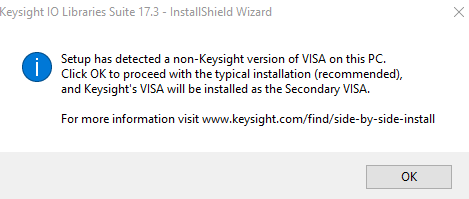
\includegraphics[scale=0.80]{keysight_visa_popup.png}
        \caption{Keysight VISA detection pop-up.}
        \label{fig:keysight_visa_popup}
        \end{center}
    \end{figure}
    \item Choose ``Custom'', then press next.
    \item Ensure the ``Install Keysight VISA as sprimary VISA.'' is checked, then press next.
    \item Press install, then wait for it to complete installation (this will take several minutes).
    \item If an error pop-up appears, as seen in \ref{fig:keysight_install_error_popup}, press OK.
    \begin{figure}[h]
        \begin{center}
        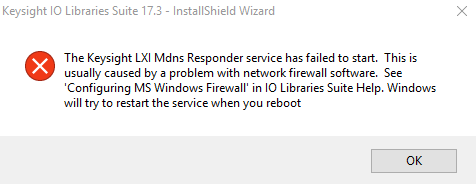
\includegraphics[scale=0.80]{keysight_install_error_popup.png}
        \caption{Keysight error pop-up during installation of IO Libraries Suite.}
        \label{fig:keysight_install_error_popup}
        \end{center}
    \end{figure}
    \item Press finish, then restart the computer.
\end{enumerate}
%%%%%%%%%%%%%%%%%%%%%%%%%%%%%%%%%%%%%%%%%%%%%%%%%%%%%%%%%%%%%%%%%%%%%%%%%%%%%%%
\subsection{AutoIt} \label{autoit} % 1.6
AutoIt is a scripting language developed to use Windows features to automate GUIs.
%%%%%%%%%%%%%%%%%%%%%%%%%%%%%%%%%%%%%%%%%%%%%%%%%%%%%%%%%%%%%%%%%%%%%%%%%%%%%%%
\subsubsection{Downloads} % 1.6.1
Download AutoIt Full Installation (top option in the downloads table) from \href{https://www.autoitscript.com/site/autoit/downloads/}{here}.
%%%%%%%%%%%%%%%%%%%%%%%%%%%%%%%%%%%%%%%%%%%%%%%%%%%%%%%%%%%%%%%%%%%%%%%%%%%%%%%
\subsubsection{Install Guide} % 1.6.2
\begin{enumerate}
    \item Run the setup file which was downloaded.
    \item Select ``Yes'' to administrator privileges.
    \item Select ``Next''.
    \item Select ``I Agree''.
    \item Select ``Use native x64 tools by default''.
    \item Select ``Next''.
    \item Select ``Run the script''.
    \item Select ``Next'', twice.
    \item Select ``Install''.
    \item Wait for the installation to complete.
    \item Uncheck ``Show release notes'', then select ``Finish''.
\end{enumerate}
%%%%%%%%%%%%%%%%%%%%%%%%%%%%%%%%%%%%%%%%%%%%%%%%%%%%%%%%%%%%%%%%%%%%%%%%%%%%%%%
\newpage
\section{Hardware Operation} % 2
This section details the setup of different hardware devices for use with the computer.
This does not cover laser usage, as this is beyond the scope of the guide and requires proper safety and equipment training.
%%%%%%%%%%%%%%%%%%%%%%%%%%%%%%%%%%%%%%%%%%%%%%%%%%%%%%%%%%%%%%%%%%%%%%%%%%%%%%%
\subsection{Supported Devices} % 2.1
\begin{itemize}
    \item ThorLabs PRM1Z8 DC Servo/Rotation Stage
    \item Newport 1918-R Handheld Optical Power Meter
    \item Meadowlark D3050 Four Channel Digital Interface
    \item Zaber T-NA08A25 Linear Actuator
    \item Newport 1830-C Optical Power Meter
    \item Princeton Instruments Spectrometer and CCD Camera
\end{itemize}
%%%%%%%%%%%%%%%%%%%%%%%%%%%%%%%%%%%%%%%%%%%%%%%%%%%%%%%%%%%%%%%%%%%%%%%%%%%%%%%
\subsection{ThorLabs PRM1Z8 DC Servo} % 2.2
The ThorLabs PRM1Z8 is a DC servo motor which can be used as a rotation stage with different optics mounted inside.
A current example of usage is with a linear polarizing filter in order to measure the polarization of the laser outputs.
%%%%%%%%%%%%%%%%%%%%%%%%%%%%%%%%%%%%%%%%%%%%%%%%%%%%%%%%%%%%%%%%%%%%%%%%%%%%%%%
\subsubsection{Setup} % 2.2.1
\begin{enumerate}
    \item Ensure you have the following required items:
    \begin{itemize}
        \item ThorLabs TCH002 Controller Hub
        \item ThorLabs TCH002 Controller Hub Power Supply
        \item 3-pin Power Cable (for power supply)
        \item Male to Male USB2 Type-A to USB2 Type-B Cable
        \item ThorLabs TDC001 DC Servo Motor Controller
        \item ThorLabs PRM1Z8 DC Servo
        \item Optics Table Mounting Equipment
    \end{itemize}
    \item Install the motor controller onto the controller hub.
    \item Connect the controller hub to the power supply.
    \item Connect the controller hub to the computer via USB.
    \item Mount the controller hub to the optics table in a convenient location.
    \item Mount the PRM1Z8 servo to the optics table as desired.
    \item Connect the servo to the motor controller.
\end{enumerate}
%%%%%%%%%%%%%%%%%%%%%%%%%%%%%%%%%%%%%%%%%%%%%%%%%%%%%%%%%%%%%%%%%%%%%%%%%%%%%%%
\subsection{Newport 1918-R Handheld Optical Power Meter} % 2.3
The Newport 1918-R handheld optical power meter is a compact optical power meter with an LCD display.
It is useful for measuring the power output of the laser.
%%%%%%%%%%%%%%%%%%%%%%%%%%%%%%%%%%%%%%%%%%%%%%%%%%%%%%%%%%%%%%%%%%%%%%%%%%%%%%%
\subsubsection{Setup} % 2.3.1
\begin{enumerate}
    \item Ensure you have the following required items:
    \begin{itemize}
        \item Newport 1918-R Handheld Optical Power Meter
        \item Newport 1918-R Handheld Optical Power Meter Power Supply
        \item Newport Optical Power Sensor
        \item Male to Male USB Mini-b to USB2 Type-A Cable
        \item Optics Table Mounting Equipment
    \end{itemize}
    \item Connect the sensor to the power meter.
    \item Connect the power supply to the power meter.
    \item Connect the power meter to the computer via USB.
    \item Mount the optical power meter sensor as desired.
\end{enumerate}
%%%%%%%%%%%%%%%%%%%%%%%%%%%%%%%%%%%%%%%%%%%%%%%%%%%%%%%%%%%%%%%%%%%%%%%%%%%%%%%
\subsection{Meadowlark D3050 Four Channel Digital Interface} % 2.4
The Meadowlark D3050 four channel digital interface is a controller which is used to control up to four Meadowlark liquid crystal devices.
This can be used to control an LCVR in the laser beam path, changing the power and polarization of the beam.
%%%%%%%%%%%%%%%%%%%%%%%%%%%%%%%%%%%%%%%
\subsubsection{Setup} % 2.4.1
\begin{enumerate}
    \item Ensure you have the following required items:
    \begin{itemize}
        \item Meadowlark D3050 Four Channel Digital Interface
        \item Meadowlark D3050 Four Channel Digital Interface Power Supply
        \item Female to Male RS232 Serial Port Cable
        \item Zaber T-USB Serial to USB Converter
    \end{itemize}
    \item Connect the power supply to the controller.
    \item Connect the controller to the serial to USB converter via RS232.
    \item Connect the serial to USB converter to the computer.
    \item Connect liquid crystal devices to the controller as desired.
\end{enumerate}
%%%%%%%%%%%%%%%%%%%%%%%%%%%%%%%%%%%%%%%%%%%%%%%%%%%%%%%%%%%%%%%%%%%%%%%%%%%%%%%
\subsection{Zaber T-NA08A25 Linear Actuator} % 2.5
The Zaber T-NA08A25 linear actuator is a linear actuator with up to 25mm of travel distance, using either manual or computer control.
This can be used to change the position of optics, and multiple devices can be daisy chained to a single computer port.
%%%%%%%%%%%%%%%%%%%%%%%%%%%%%%%%%%%%%%%
\subsubsection{Setup} % 2.5.1
\begin{enumerate}
    \item Ensure you have the following required items:
    \begin{itemize}
        \item Zaber T-NA08A25 Linear Actuator
        \item Zaber T-NA08A25 Linear Actuator Power Supply
        \item Zaber T-USB Serial to USB Converter
        \item Zaber Mini-DIN to 9-Pin Serial Adapter
    \end{itemize}
    \item Connect the power supply to the linear actuator(s).
    \item Connect the linear actuators to each other if using more than one.
    \item Connect the actuator to the Mini-DIN to 9-Pin serial adapter.
    \item Connect the Mini-DIN to 9-Pin serial adapter to the serial to USB converter.
    \item Connect the serial to USB adapter to the computer.
\end{enumerate}
%%%%%%%%%%%%%%%%%%%%%%%%%%%%%%%%%%%%%%%%%%%%%%%%%%%%%%%%%%%%%%%%%%%%%%%%%%%%%%%
\subsection{Newport 1830-C Optical Power Meter} % 2.6
The Newport 1830-C optical power meter is a desktop optical power meter which uses photodiode sensors to take optical power measurements.
This can be used to calibrate the laser input power, and to monitor the power during experimentation.
%%%%%%%%%%%%%%%%%%%%%%%%%%%%%%%%%%%%%%%%%%%%%%%%%%%%%%%%%%%%%%%%%%%%%%%%%%%%%%%
\subsubsection{Setup} % 2.6.1
\begin{enumerate}
    \item Ensure you have the following required items:
    \begin{itemize}
        \item Newport 1830-C Optical Power Meter
        \item Newport Optical Power Sensor
        \item Agilent GPIB-USB Converter Cable
    \end{itemize}
    \item Connect the optical power meter to power.
    \item Connect the GPIB-USB cable to the optical power meter and computer.
    \item Connect the optical power sensor to the optical power meter.
    \item Mount the optical power sensor in the beam path.
\end{enumerate}
%%%%%%%%%%%%%%%%%%%%%%%%%%%%%%%%%%%%%%%%%%%%%%%%%%%%%%%%%%%%%%%%%%%%%%%%%%%%%%%
\subsection{Princeton Instruments Spectrometer and CCD Camera} % 2.7
The Princeton Instruments Spectrometer and CCD Camera require LightField to be installed in order to function.
The full initial setup is detailed from Princeton documentation, this section will deal with setup required to use the equipment after initial setup.
%%%%%%%%%%%%%%%%%%%%%%%%%%%%%%%%%%%%%%%%%%%%%%%%%%%%%%%%%%%%%%%%%%%%%%%%%%%%%%%
\subsubsection{Setup} % 2.7.1
\begin{enumerate}
    \item Ensure that the CCD and Spectrometer are connected to the computer.
    \item Power on the CCD and Spectrometer by switching their power supplies on.
    \item Open LightField and check that the devices are detected.
\end{enumerate}
%%%%%%%%%%%%%%%%%%%%%%%%%%%%%%%%%%%%%%%%%%%%%%%%%%%%%%%%%%%%%%%%%%%%%%%%%%%%%%%
\newpage
\section{Software Operation} % 3
REMOVED FOR PUBLIC CONSUMPTION
%%%%%%%%%%%%%%%%%%%%%%%%%%%%%%%%%%%%%%%%%%%%%%%%%%%%%%%%%%%%%%%%%%%%%%%%%%%%%%%
\newpage
\section{Troubleshooting} % 4
This section is intended to give general advice to troubleshooting problems which may arise.
%%%%%%%%%%%%%%%%%%%%%%%%%%%%%%%%%%%%%%%%%%%%%%%%%%%%%%%%%%%%%%%%%%%%%%%%%%%%%%%
\subsection{General Advice} % 4.1
General device can be used to approach any problem which does not have a specific solution in the guide.
These techniques are also useful when troubleshooting software and hardware outside of the lab.
\begin{itemize}
    \item Check the all the power and data connections are properly secured, and try unplugging/replugging them back in.
    \item Try restarting the computer.
    \item Check in ``Device Manager'' that there are no yellow warning triangles for devices, and that the devices drivers are installed correctly.
    \item Attempt to reinstall the device drivers/programs as this can fix problems with the .dll's which are used.
        \subitem An exception to this is the Python installation.
        Unless there is a missing import error, there is no need to reinstall Anaconda or any packages.
\end{itemize}
%%%%%%%%%%%%%%%%%%%%%%%%%%%%%%%%%%%%%%%%%%%%%%%%%%%%%%%%%%%%%%%%%%%%%%%%%%%%%%%
\subsection{Specific Error Solutions} % 4.2
Specific error solutions are errors which have come up in the lab which may arise in the future.
This will not cover any problems arising from bugs in the program source code.
If there is a bug in the source code, it is wise to make a backup before changing any code.
If you fix the error, document the correction and source code change, and ensure that it doesn't change the function of the program.
%%%%%%%%%%%%%%%%%%%%%%%%%%%%%%%%%%%%%%%%%%%%%%%%%%%%%%%%%%%%%%%%%%%%%%%%%%%%%%%
\subsubsection{thorlabs\_apt [WinError 126]} % 4.2.1
This error arises when thorlabs\_apt cannot find the ``APT.dll'' which is installed with the APT 32-bit for 64-bit installation.
An example of this error can be seen in Figure \ref{fig:missing_aptdll}.
\begin{figure}[h]
    \begin{center}
    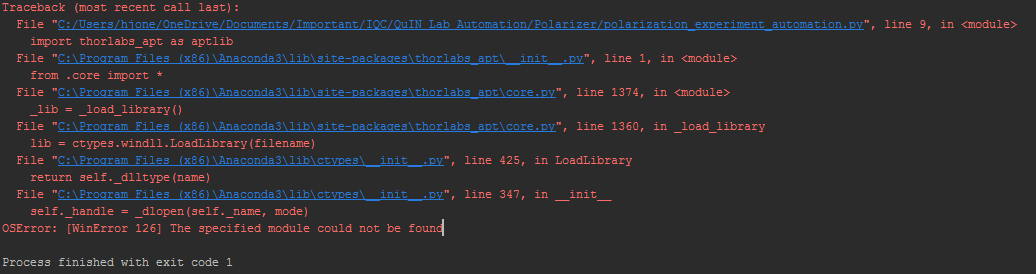
\includegraphics[scale=.60]{missing_aptdll.png}
    \caption{[WinError 126] caused by thorlabs\_apt being unable to find ``APT.dll''.}
    \label{fig:missing_aptdll}
    \end{center}
\end{figure}
\\Solution:
\begin{enumerate}
    \item Open Windows Explorer and navigate to ``C:\textbackslash Program Files (x86)\textbackslash Thorlabs\textbackslash APT\textbackslash APT Server''.
    \item Copy ``APT.dll''.
    \item Open the directory where the source code is running from, and paste these files into that directory.
    \item Open ``C:\textbackslash Program Files (x86)\textbackslash Anaconda3\textbackslash Lib\textbackslash site-packages\textbackslash thorlabs\_apt''.
    \item Paste the files in this directory.
\end{enumerate}
The program should now run correctly.
%%%%%%%%%%%%%%%%%%%%%%%%%%%%%%%%%%%%%%%%%%%%%%%%%%%%%%%%%%%%%%%%%%%%%%%%%%%%%%%
\newpage
\section{Programming} % 5
This section of the guide is to provide tips on programming and documentation in Python for usage in QuIN Lab.
%%%%%%%%%%%%%%%%%%%%%%%%%%%%%%%%%%%%%%%%%%%%%%%%%%%%%%%%%%%%%%%%%%%%%%%%%%%%%%%
\subsection{Documentation} % 5.1
All of the code which is created for usage within QuIN Lab should be documented use the NumPy documentation guidelines.
These guidelines can be found \href{https://github.com/numpy/numpy/blob/master/doc/HOWTO_DOCUMENT.rst.txt}{here}.
%%%%%%%%%%%%%%%%%%%%%%%%%%%%%%%%%%%%%%%%%%%%%%%%%%%%%%%%%%%%%%%%%%%%%%%%%%%%%%%
\subsection{Style} % 5.2
All of the code which is created for usage within QuIN Lab should follow the Python PEP8 Style guide.
The PEP8 style guide can be found \href{https://www.python.org/dev/peps/pep-0008/}{here}.
%%%%%%%%%%%%%%%%%%%%%%%%%%%%%%%%%%%%%%%%%%%%%%%%%%%%%%%%%%%%%%%%%%%%%%%%%%%%%%%
\subsection{wxPython Phoenix} % 5.3
All of the wxPython Phoenix documentation is available \href{https://wxpython.org/Phoenix/docs/html/main.html}{here}.
Additionally, it is recommended to try searching for your problem online, as wxPython and wxPython Phoenix are used quite commonly.
There is likely a solution to your problem already.

When programming a GUI, it is important to use a different thread for the automation, which is a subthread of the GUI thread.
To make this threading work, the GUIs use \_thread to run the automation.
It is very important that any calls to methods or objects which change the GUI appearance must use wx.CallAfter(method, parameters), otherwise the automation and GUI will not work properly.
It is also very important when programming, to make sure that objects have proper parents, otherwise the GUI can look very unusable.
%%%%%%%%%%%%%%%%%%%%%%%%%%%%%%%%%%%%%%%%%%%%%%%%%%%%%%%%%%%%%%%%%%%%%%%%%%%%%%%
\end{document}
